\documentclass[10pt,a4paper]{article}

\usepackage[margin=0.3in]{geometry} 

\usepackage{graphicx}
\graphicspath{ {images/} }

% Make the titles smaller
% \usepackage[compact]{titlesec}
% \titleformat*{\section}{\normalsize\bfseries\scshape}
% \titleformat*{\subsection}{\small\bfseries}

\usepackage{multicol}
\setlength{\columnseprule}{0.4pt} % Divide size

\begin{document}
	\begin{multicols}{3}

	\section{Meme}

	 \begin{figure}[h!]
	    \centering
	    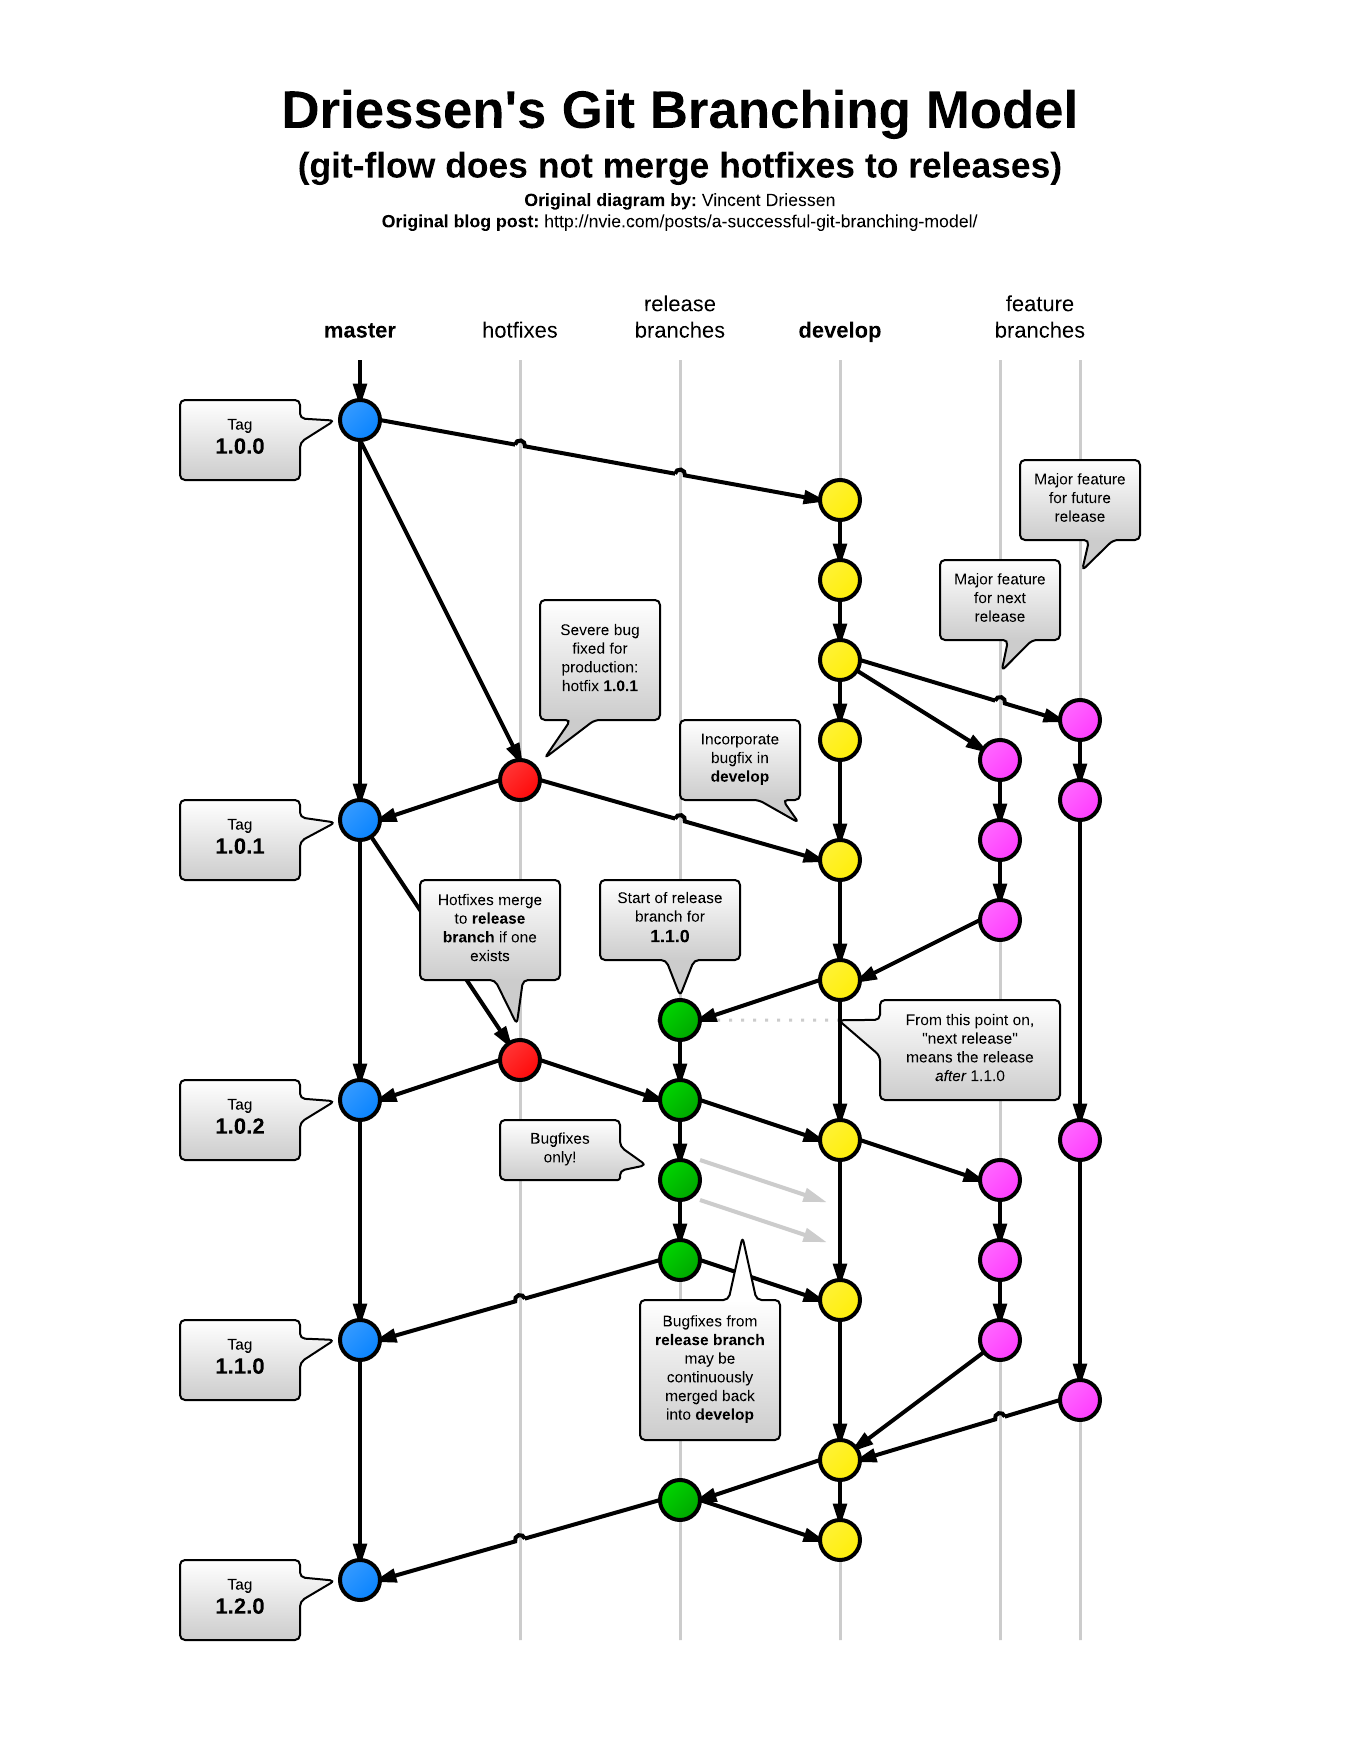
\includegraphics[width=0.7\textwidth]{git-flow-flipped.png}
	 \end{figure}
	
	 \subsubsection{Libraries}\label{libraries}

Dropwizard uses - Jetty for HTTP - Jersey for REST - Jackson for JSON -
Metrics for metrics - Guava for utilities - SL4J \& Logback for logging
- JDBI for datastorage

Apache Derby - Small footprint - Based on the Java, JDBC, and SQL

Flyway - ``Evolve your Database Schema easily and reliably across all
your instances''

Kyrnonet - ``\ldots{} a clean and simple API for efficient TCP and UDP''
- Makes use of the Kryo Serialisation Library

\subsubsection{Toooling}\label{toooling}

Jenkins - Continuous integration server SonarQube - Code quality JUnit -
Test framework JaCoCo - Test coverage Gradle - Build automation system
Artifactory - single access point to binary resources

\subsubsection{TDD}\label{tdd}

\begin{itemize}
\item
  When you get a bug report, write a test that exposes the bug
\item
  Concentrate tests on \emph{boundary conditions}.
\item
  Test for \emph{exceptional behaviours}.
\end{itemize}

\subsubsection{Git}\label{git}

Central repository • Pull master branch • Edit, stage, commit to local
master • Push to central repository

Distributed repositories • Each developer has their own repository •
Work on local master • Use pull requests to notify of code to merge •
Repository manager approves and pulls code to main repo

Release branches • Each release \& patch is its own branch • Simplifies
maintaining multiple versions of a system • Separate master for releases
• Development happens in branches • Simplified history of releases • Bug
fixes • Branches for bug fixes • Merged into master when fixed

\subsubsection{Mocking}\label{mocking}

\begin{itemize}
\item
  Dummies - test objects which are never used but exist only to satisfy
  syntactic requirements -- Stubs - test objects whose methods return
  fixed values, and support the specific test cases only
\item
  Fakes --- test objects whose methods work but have only limited
  functionality -- Mocks --- test objects which know how they're meant
  to be used, e.g.~the sequence in which their methods should be called
  (allowing behavioural verification instead of just state verification)
\end{itemize}

\subsubsection{Databases}\label{databases}

JDBC -- Java Database Connectivity - Is a built-in Java library that
enables direct programmatic control over a relational database, without
needing to use SQL - Provides methods for querying and updating data in
the database - Oriented towards relational database - Low level control
- Java library, therefore Does NOT require third party imports - Client
side drivers convert from java to DBMS protocol - More lines of code,
faster at run time

JDBI -- intermediate level relational database library - Like JDBC, but
also provides simple tools for DAO's (Data Access Objects) - Methods
access DAO connected to underlying database. - Low-level control -
Simplified usage compared to JDBC, slower in execution

JPA -- Java Persistence API -- more advanced Data Access Object tools -
JPA is an object-role modelling approach to working with a database from
a Java program. - The idea is that in the program you focus on objects.
- In the database you design your tables, relations, keys and
constraints. - You then specify how to map from the program's objects to
the database's tables.

JDO -- similar in concept to JPA, but is not limited to relational
databases. - Allows changes to underlying DB technology (more control) -
Supports NoSQL and other database structures other than RDB



   	\end{multicols}
\end{document}